\documentclass[10pt]{article}
\usepackage[margin=1in]{geometry}
\usepackage[T1]{fontenc}
\usepackage{amsmath,amssymb}
\usepackage{graphicx}
\usepackage{booktabs}
\usepackage{hyperref}
\usepackage{caption}
\usepackage{float}
\captionsetup{font=small}
\setlength{\parskip}{4pt}

\title{\textbf{abkit: A/B Test Analysis That Has Been Stress Tested,\\Cross Checked, and Applied to a Real Experiment}}
\author{Matin Nikoomanzar\\University of California, Los Angeles\\\small\url{https://github.com/MatinNikoo/abkit}}
\date{October 2026}

\begin{document}
\maketitle

\begin{abstract}
\noindent Online experiments are simple in principle, but a few common problems quietly make their results wrong, namely checking results repeatedly, noisy metrics, ratio metrics, rows that aren't independent, broken or uneven assignment, and testing many things at once. abkit is an open source Python library and command line tool that handles each one with established methods, and this paper asks a narrower question about them, which is \emph{do they keep their stated error rates on data that looks like real product metrics, and where they don't, what is the smallest fix?} I test every method on simulated experiments with a known answer, across 127 combinations of method and data, with conditions that include skewed and heavy tailed revenue, zero inflated spend, conversion rates down to 0.1\%, sessions nested in users, clustered randomization, four kinds of missing data, and effects that vary by user, and I check every estimator against scipy, statsmodels and published tables. The stress tests found two real bugs in the sequential test, both fixed, and three findings worth knowing. Skewed revenue only breaks the $t$ test when group sizes are uneven (11.4\% false positives at 1,000 vs 19,000 users, almost all on one side, against 3.9\% with equal groups); a row level test on 50 randomized clusters per group gives 41.7\% false positives; and a split check that counts users in a clustered test flags 73.7\% of healthy experiments. Applied to a public mobile game experiment with 90,189 players, the library flags a sample ratio mismatch ($p = 0.009$). A placebo built from the game design shows that most of the imbalance sits in players who played too few rounds to reach the treatment. The 7 day retention drop keeps its direction under every reading, and in the subgroup with a clean split the $p$ value rises from 0.0016 to 0.07, mostly because that subgroup holds only 38\% of the players and its estimated drop is slightly larger (0.97 vs 0.82 points).
\end{abstract}

\section{Introduction}
Product teams decide what to ship by running randomized experiments. The textbook analysis is a two sample test at a sample size chosen in advance. In practice that analysis is often wrong for reasons that have nothing to do with the math of the $t$ test. People check dashboards daily and stop when the result looks good. Metrics are noisy and skewed. Metrics like clicks per session are ratios whose denominator is not the unit that was randomized. Assignment and logging bugs produce uneven splits. A dashboard of twenty metrics will usually show at least one false win.

None of these problems are new, and each has a known fix in the literature. The first version of abkit put those fixes in one small library and checked each one on clean simulated data. This version asks whether the fixes survive messy data, and adds the methods a large experimentation team would expect, which are group sequential designs, cluster robust and randomization inference, regression adjustment with separate slopes, model based covariates with cross fitting, power calculations for ratio metrics, tools for skewed metrics, non-inferiority tests for guardrail metrics, and checks for effects that change over time.

The research question is falsifiable on purpose. A method passes a condition when its simulated false positive rate is not above 5\% by more than two Monte Carlo standard errors, its 95\% interval covers the truth at least 95\% of the time minus two standard errors, and neither tail takes more than its 2.5\% share of the errors. Every number in this paper comes from scripts in the repository, and the full table of 127 rows is in \texttt{docs/validation.md}.

\section{Methods}
Throughout, $Y$ is a user level outcome, $C$ and $T$ index control and treatment, and $\Delta = \mu_T - \mu_C$.

\paragraph{Difference in means.} The default test is Welch's $t$ test with Welch Satterthwaite degrees of freedom. Binary outcomes are handled as means of 0/1 values. The relative lift $\bar Y_T/\bar Y_C - 1$ gets its interval from the delta method,
\[ \operatorname{Var}\!\left(\frac{\bar Y_T}{\bar Y_C}\right) \approx \frac{\operatorname{Var}(\bar Y_T)}{\bar Y_C^2} + \frac{\bar Y_T^2 \operatorname{Var}(\bar Y_C)}{\bar Y_C^4}. \]

\paragraph{A skewness diagnostic for two groups.} Kohavi et al.\ (2014) suggest $n > 355 s^2$ users for a mean with skewness $s$, which is the same as asking that the mean's own skewness $s/\sqrt n$ stay under $1/\sqrt{355}$. For a difference of two means with a common shape, the third cumulant is $\kappa_3(1/n_T^2 - 1/n_C^2)$, so the skewness of the difference is
\[ \gamma_\Delta = s\,\frac{n_T^{-2} - n_C^{-2}}{(n_C^{-1} + n_T^{-1})^{3/2}}, \]
which is exactly zero when $n_C = n_T$. abkit estimates $s$ from both groups pooled and attaches a note to the result when $|\gamma_\Delta| > 1/\sqrt{355}$. Section~\ref{sec:stress} shows this is the condition under which the $t$ test actually breaks.

\paragraph{Ratio metrics and clusters.} For a metric $\sum_i X_i / \sum_i N_i$ with one row per user, the delta method variance (Deng, Knoblich and Lu, 2018) is $\operatorname{Var}(Z)/(n \mu_N^2)$ with linearized values $Z_i = X_i - r N_i$. When rows come in clusters (sessions of a user, randomized cities), \texttt{cluster\_test} sums rows per cluster and applies the same formula, which equals a cluster robust standard error times $G/(G-1)$. It uses a $t$ reference with Welch degrees of freedom counted in clusters, and optionally a randomization test that reshuffles the cluster labels and recomputes the studentized statistic, which is exact for the sharp null that treatment changes no cluster's outcome and, because the statistic is studentized, approximately valid for the null of no average effect.

\paragraph{Regression adjustment.} CUPED (Deng, Xu, Kohavi and Walker, 2013) analyzes $Y - \theta^\top(X - \bar X)$ with $\theta$ the pooled least squares slope, which removes about $\rho^2$ (or $R^2$) of the variance. \texttt{adjusted\_test} fits a separate slope in each group, centered at the pooled covariate mean (Lin, 2013). When users are a sample from a larger population, its variance needs a term the usual robust standard error leaves out, $(\theta_T - \theta_C)^\top \Sigma_X (\theta_T - \theta_C)/N$; without it the simulated false positive rate was about 7\%. CUPAC uses a model's prediction from many pre period features as the covariate. To keep the prediction for a user independent of that user's outcome, \texttt{cupac\_adjust} cross fits, so each fold is predicted by a model trained on the other folds, never on the assignment.

\paragraph{Sample ratio mismatch.} A chi square goodness of fit test compares the observed counts of the randomized unit with the intended split (Fabijan et al., 2019). A small $p$ value is a reason to investigate. It does not establish a fault, since one healthy test in a hundred falls below 0.01.

\paragraph{Sequential testing.} The mixture sequential probability ratio test (Johari, Koomen, Pekelis and Walsh, 2017) uses, for an estimate $\hat\Delta_n$ with variance $V_n$ and a mixture $\Delta \sim N(0,\tau^2)$,
\[ \Lambda_n = \sqrt{\frac{V_n}{V_n + \tau^2}}\,\exp\!\left(\frac{\tau^2 \hat\Delta_n^2}{2 V_n (V_n + \tau^2)}\right), \]
with always valid $p_n = \min_{k \le n} \min(1, 1/\Lambda_k)$ and the matching confidence sequence (Howard et al., 2021), intersected over time. $V_n$ is plugged in from the data. Looks where either group has zero sample variance are skipped (Section~\ref{sec:bugs}). Group sequential designs fix the number of looks in advance. abkit computes two sided boundaries by recursive numerical integration of the score process (Armitage, McPherson and Rowe, 1969) for O'Brien and Fleming (1979) and Pocock (1977) shapes, and for the Lan and DeMets (1983) spending functions $\alpha(t) = 4\left(1 - \Phi\!\left(z_{1-\alpha/4}/\sqrt t\right)\right)$ and $\alpha \log(1 + (e-1)t)$. Repeated confidence intervals are $\hat\Delta_k \pm b_k \mathrm{SE}_k$.

\paragraph{Other tools.} Holm and Benjamini Hochberg corrections; Dunnett comparisons of several treatments with one control using the multivariate normal with correlations from the shared control and unequal variances; Cochran's $Q$ for segment heterogeneity and a screen that applies it to many user traits with a false discovery rate correction; a Bayesian chance to win with an optional normal prior on the lift; percentile and studentized bootstrap intervals; quantile effects; the Mann-Whitney probability of superiority with the Brunner and Munzel (2000) variance; one sided non-inferiority tests; and a weighted trend test and a weekday $Q$ test on daily lifts.

\section{Verification beyond simulation}
A simulation can only show that a method behaves as I expect. To catch mistakes in my expectations, every estimator is also checked against an independent implementation or a published number in \texttt{tests/\allowbreak test\_reference.py}. Welch intervals match scipy and statsmodels to $10^{-10}$; the cluster delta method matches statsmodels' cluster robust OLS exactly after the $G/(G-1)$ factor; the CUPED slope matches OLS; the separate slopes estimator matches the interacted regression coefficient; Holm and Benjamini Hochberg match statsmodels and reproduce the 15 $p$ value example of Benjamini and Hochberg (1995); the classic group sequential constants match Jennison and Turnbull (2000) (Pocock 2.413, O'Brien Fleming 2.040 for five looks, and the inflation factors) and the spending boundaries match gsDesign (4.877, 3.357, 2.680, 2.290, 2.031); the Beta chance to win matches numerical integration; and the sample ratio test reproduces a textbook example ($p \approx 1.8\times 10^{-6}$ for 821,588 vs 815,482). Property based tests (hypothesis) check invariances on simulated data. Swapping groups flips the sign, shifting and scaling leave $p$ unchanged, $p$ values stay in $[0, 1]$ and never rise in the sequential test, intervals contain the estimate and widen as $\alpha$ falls. One of these found a cancellation problem in the ratio variance. The test suite has 188 tests and runs on Python 3.10 to 3.13.

\section{The original simulation study}
Table~\ref{tab:sim} repeats the checks from the first version on clean data. The numbers are unchanged after the fixes in this version.

\begin{table}[!tb]
\centering\small
\begin{tabular}{p{4.6cm}p{9.6cm}}
\toprule
Check & Result \\
\midrule
Peeking, 2{,}000 A/A tests, 100 looks & Ordinary p value: 20.6\% false positives by look 10, 39.4\% by look 100. mSPRT: 2.2\%. \\
Power, 500 tests per effect size & Effect 0.04 sd: 52\% (mSPRT) vs 81\% (single look). Effect 0.06 sd: 92\% vs 99\%, with mSPRT stopping after 45\% of the sample on average. \\
CUPED variance reduction & Measured 9\%, 25\%, 49\%, 81\% at $\rho = 0.3, 0.5, 0.7, 0.9$, matching $\rho^2$. \\
CUPED interval coverage & 94\% to 96\% at every $\rho$ (nominal 95\%). Power at $\rho = 0.7$ rose from 62\% to 89\%. \\
Two covariates vs one & 50\% vs 25\% of the variance removed, matching $R^2$. \\
Ratio metric coverage & Delta method 96.2\%, sessions treated as independent 88.0\%. \\
Sample size formula & Promised 80\% power, achieved 82\%, 80\%, 79\%. \\
20 metrics, 15 null & Any false win: 53\% uncorrected, 4.4\% Holm. Benjamini Hochberg false discovery rate 3.8\%. \\
Chance to win, tiny true effects & Flat prior: stated 85\%, right 73\% of the time. Prior matched to past effects: stated 85\%, right 86\%. \\
10 segments, no effect anywhere & Some segment significant: 41\% uncorrected, 5.8\% with Benjamini Hochberg. Cochran's Q false alarm rate 6.1\%. \\
\bottomrule
\end{tabular}
\caption{Clean data simulations (\texttt{simulations/run\_simulations.py}).}
\label{tab:sim}
\end{table}

\section{Stress tests}\label{sec:stress}
\texttt{simulations/stress.py} runs 22 scenarios, each with 2,000 experiments without an effect and 1,000 with one, so the Monte Carlo standard error is about 0.5 points on a 5\% rate and 0.7 points on 95\% coverage. Table~\ref{tab:stress} shows the $t$ test on a selection; Figure~\ref{fig:stress} shows every scenario.

\begin{table}[!tb]
\centering\scriptsize
\begin{tabular}{p{4.3cm}rrrp{4.4cm}}
\toprule
Data & Type I (\%) & lower / upper tail & Coverage (\%) & Alternative: Type I, coverage \\
\midrule
normal, 2,000 per group & 4.8 $\pm$ 0.5 & 2.1 / 2.6 & 96.1 $\pm$ 0.6 &  \\
lognormal sd 2, 2,000 per group & 3.9 $\pm$ 0.4 & 2.1 / 1.7 & 94.2 $\pm$ 0.7 & cuped: 4.5, 92.9 \\
lognormal sd 2, 1,000 vs 19,000 & 11.4 $\pm$ 0.7 & 0.1 / 11.3 & 90.2 $\pm$ 0.9 & cuped: 10.1, 95.2 \\
Pareto shape 1.5 (infinite variance), 5,000 per group & 4.0 $\pm$ 0.4 & 1.8 / 2.3 & 96.1 $\pm$ 0.6 &  \\
5\% buyers, lognormal spend, 10,000 per group & 5.5 $\pm$ 0.5 & 2.9 / 2.5 & 94.1 $\pm$ 0.7 & cuped: 5.4, 94.1 \\
0.1\% conversion, 20,000 per group & 5.0 $\pm$ 0.5 & 2.5 / 2.5 & 95.0 $\pm$ 0.7 &  \\
2,000 users per group, about 5 sessions each & 11.3 $\pm$ 0.7 & 5.7 / 5.7 & 89.8 $\pm$ 1.0 & cluster: 5.5, 94.0 \\
50 clusters per group randomized whole, ICC 0.05 & 41.7 $\pm$ 1.1 & 20.9 / 20.8 & 60.6 $\pm$ 1.5 & cluster perm: 5.4, 94.0 \\
8 clusters per group randomized whole, ICC 0.05 & 66.3 $\pm$ 1.1 & 32.9 / 33.4 & 32.1 $\pm$ 1.5 & cluster perm: 5.0, 87.9 \\
low outcomes go missing, same rule both groups & 5.1 $\pm$ 0.5 & 2.5 / 2.5 & 92.1 $\pm$ 0.9 & cuped: 5.1, 93.2 \\
treatment makes low users drop out of logging & 67.2 $\pm$ 1.0 & 0.0 / 67.2 & 39.5 $\pm$ 1.5 & cuped: 27.2, 74.9 \\
effect varies with a pre period trait, 10/90 & 4.3 $\pm$ 0.5 & 2.6 / 1.7 & 94.7 $\pm$ 0.7 & cuped: 4.5, 95.0 \\
\bottomrule
\end{tabular}

\caption{Welch $t$ test under messy data, with the false positives split by side (each should be 2.5\%), and the alternative abkit offers where the $t$ test fails. Rates in percent $\pm$ one Monte Carlo standard error.}
\label{tab:stress}
\end{table}

\begin{figure}[!tb]
\centering
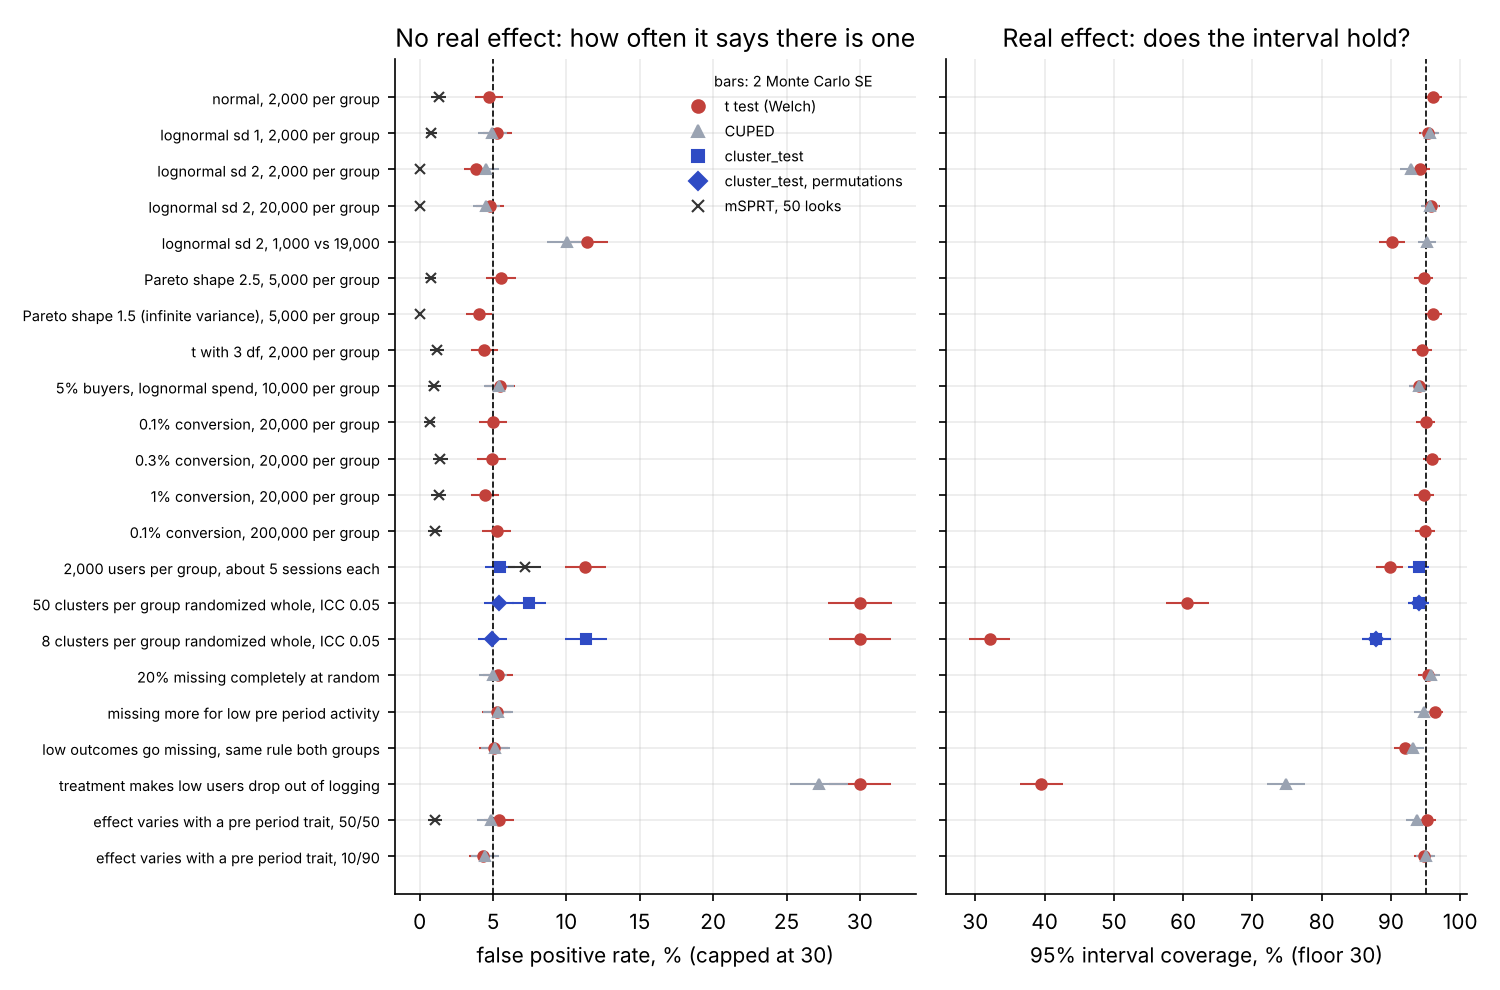
\includegraphics[width=0.92\linewidth]{../figures/stress_overview.png}
\caption{False positive rate with no effect (left) and 95\% interval coverage with an effect (right), every stress scenario. Bars are two Monte Carlo standard errors.}
\label{fig:stress}
\end{figure}

\paragraph{Skew needs uneven groups to hurt.} On lognormal revenue with sd 2 (skewness over 400) the $t$ test gave 3.9\% false positives at 2,000 users per group and 4.8\% at 20,000. With 1,000 users in control and 19,000 in treatment it gave 11.4\%, of which 11.3 points were in the upper tail and 0.1 in the lower, and its 95\% interval covered the truth 90.2\% of the time. CUPED gave 10.1\% there, the separate slopes estimator 12.2\% and the flat prior Bayesian interval 11.3\%. A 99th percentile cap gave 4.9\%, but only because it estimates a different quantity and lost 32.9\% of the true lift. Figure~\ref{fig:skew} follows the one sided errors at skewness 33. With equal groups both tails stay near 2.5\% at every size. With a 1 to 9 split the upper tail is 9.4\%, 6.3\%, 4.6\% and 3.5\% when the smaller group has 200, 1,000, 5,000 and 20,000 users, so it shrinks with $n$ but is still above 2.5\% at 20,000. The skewness note fired on every unequal test here and on no test in any of the other 21 scenarios. A bootstrap does not repair it. At 1,000 vs 9,000 users with sd 1.5, the false positive rates were 7.7\% for the $t$ test, 7.7\% for the percentile bootstrap and 6.3\% for the studentized bootstrap, with coverage of 92.5\%, 92.0\% and 90.8\%.

\begin{figure}[!tb]
\centering
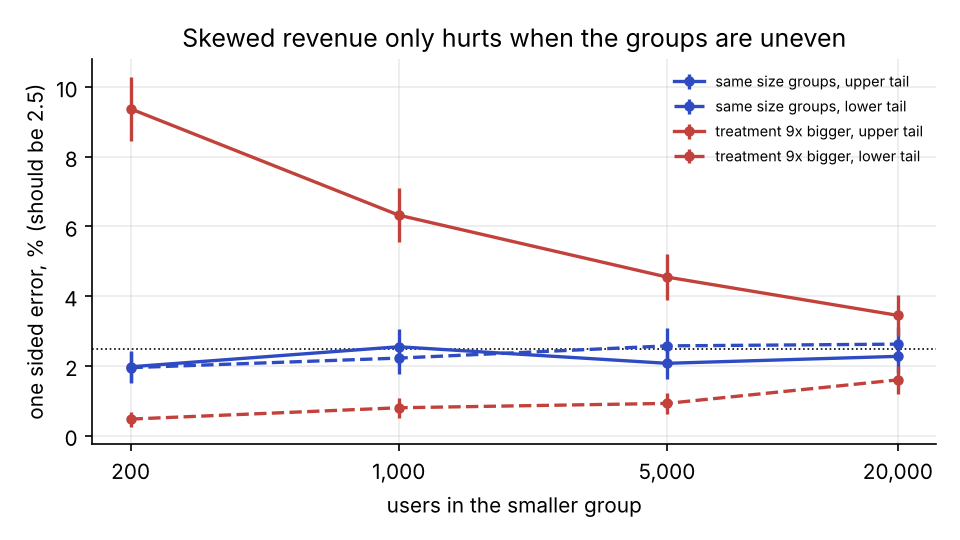
\includegraphics[width=0.62\linewidth]{../figures/stress_skew.png}
\caption{One sided error rates for lognormal revenue (skewness 33) as the smaller group grows. The Kohavi et al.\ rule asks for about 400,000 users per group here; with equal groups the $t$ test is fine at 200.}
\label{fig:skew}
\end{figure}

\paragraph{Rare events alone are fine.} At 0.1\%, 0.3\% and 1\% conversion with 20,000 users per group, and 0.1\% with 200,000, the $t$ test gave 5.0\%, 4.9\%, 4.5\% and 5.2\% false positives with coverage between 94.8\% and 95.9\%. Heavy tails keep the error rates too. With Pareto shape 2.5 it was 5.5\% and 94.7\%, and with infinite variance (shape 1.5) 4.0\% and 96.1\%, but the power fell from 84.2\% to 30.4\%. The test stays valid and loses its ability to find anything. The sequential test is where rare events did cause trouble before the fix in Section~\ref{sec:bugs}. Afterwards its confidence sequence covered the truth 98.7\% of the time at 0.1\% conversion with no empty intervals.

\paragraph{Clusters.} With 2,000 users per group and about five sessions each, analyzing sessions as if they were independent gave 11.3\% false positives and 89.8\% coverage. \texttt{cluster\_test} gave 5.5\% and 94.0\%. The mSPRT run on rows had 7.1\% false positives, so the sequential tests share the problem. Randomizing 50 clusters per group with an intraclass correlation of 0.05 and uneven cluster sizes pushed a row level test to 41.7\% false positives and 60.6\% coverage. \texttt{cluster\_test} gave 7.4\%, with 4.0\% in the upper tail, and the randomization version with 999 permutations gave 5.4\%. With 8 clusters per group the three were 66.3\%, 11.3\% and 5.0\%, but the interval from the permutation version is still the $t$ interval and covered only 87.9\%. Counting rows in the split check is a trap of its own. At the 0.01 level it flagged 73.7\% of healthy experiments with 50 clusters per group and 87.3\% with 8, while counting clusters flagged none. The A/A simulator in \texttt{aa\_test} shows the same thing on a user's own data. Splitting users and testing rows gave 12.5\% false positives, testing clusters gave 4.7\%.

\paragraph{Missing data.} Twenty percent missing completely at random, or missing more for users with low pre period activity, did no harm (5.3\% and 5.2\% false positives, coverage 95.3\% and 96.4\%). When low outcomes go missing under the same rule in both groups the false positive rate stays at 5.1\%, but the estimate is 20.8\% too small and coverage drops to 92.1\%. CUPED is off by 7.5\%. The missing value check noticed in only 12.8\% of those tests. When the treatment itself makes low users drop out of the logs, the $t$ test gave 67.2\% false positives and an estimate 75.0\% too large. CUPED still gave 27.2\% and a bias of 24.8\%. The missing value check caught this case in 93.0\% of tests, but nothing in the analysis can correct it afterwards.

\paragraph{Effects that vary by user.} When the effect depends on a pre period trait, nothing breaks. With a 50/50 split the $t$ test gave 5.4\% false positives and CUPED 4.9\%, with CUPED raising power from 59.8\% to 94.5\%. With a 10/90 split the false positive rates were 4.3\% for the $t$ test and 4.5\% for both adjusted estimators, and power was 82.2\% for the $t$ test, 95.5\% for pooled slope CUPED and 98.5\% for the separate slopes estimator.

\section{Two bugs the stress tests found}\label{sec:bugs}
\textbf{Precision.} The running variance in the sequential test came from cumulative sums of $x$ and $x^2$. For a metric whose mean is large compared with its spread (mean $10^8$, sd 1), the subtraction loses every significant digit; the test returned $p = 0$ and an interval whose ends were swapped. The data is now shifted by its first value before summing. A property based test checks shift invariance up to $10^9$.

\textbf{Collapsing confidence sequences on rare events.} At a 0.1\% conversion rate the first looks often have no conversions at all in a group, so the plug in variance is zero and the confidence sequence collapses to a point. Because the sequence is intersected over time, later looks inherit the collapse. In 600 simulated tests with 20,000 users per group and a true effect (\texttt{simulations/msprt\_rare\_events.py}), the interval missed the truth at some look 33.8\% of the time, and 11.5\% of the tests ended with an empty interval. Skipping looks where a group has no spread yet brought that to 0.7\% and 0\%. Neither fix changes any result on data where every look has some spread, including the Cookie Cats analysis.

\section{Planned looks or open ended monitoring}
Table~\ref{tab:gsd} and Figure~\ref{fig:gsd} compare a single look, the mSPRT checked 50 times, and five look group sequential designs on the same simulated experiments with 10,000 users per group. With no effect all four stay at or under 5\%, the mSPRT far under (0.9\%), because its guarantee covers any number of looks with no end date. O'Brien Fleming keeps almost all of the single look power (79.0\% vs 80.0\% at 0.04 sd) while using 81\% of the users on average at that effect. Pocock stops earliest (57\% of the users at 0.05 sd) but gives up about 9 points of power at 0.04 sd. The mSPRT, with $\tau = 0.03$, reaches 47.9\% at 0.04 sd; that is the price of being allowed to look at any time, as often as you like, with no maximum sample. Simulated power agrees with the numerical integration within two Monte Carlo standard errors at every effect size (79.0\% vs 79.8\% for O'Brien Fleming at 0.04 sd), and the repeated confidence intervals covered the truth at every look 94.1\% to 96.0\% of the time.

\begin{table}[!tb]
\centering\scriptsize
\begin{tabular}{lrrrrr|rrrrr}
\toprule
 & \multicolumn{5}{c|}{Rejection rate (\%) at effect (sd)} & \multicolumn{5}{c}{Average share of users used (\%)} \\
 & 0.0 & 0.02 & 0.03 & 0.04 & 0.05 & 0.0 & 0.02 & 0.03 & 0.04 & 0.05 \\
\midrule
Single look & 5 & 31 & 55 & 80 & 94 & 100 & 100 & 100 & 100 & 100 \\
mSPRT, 50 looks & 1 & 10 & 23 & 48 & 74 & 100 & 97 & 92 & 82 & 69 \\
O'Brien Fleming, 5 looks & 5 & 30 & 54 & 79 & 94 & 99 & 95 & 90 & 81 & 71 \\
Pocock, 5 looks & 5 & 24 & 47 & 71 & 90 & 98 & 91 & 82 & 71 & 57 \\
\bottomrule
\end{tabular}

\caption{Rejection rates and average share of the maximum sample used, 4,000 experiments without an effect and 1,000 per effect size.}
\label{tab:gsd}
\end{table}

\begin{figure}[!tb]
\centering
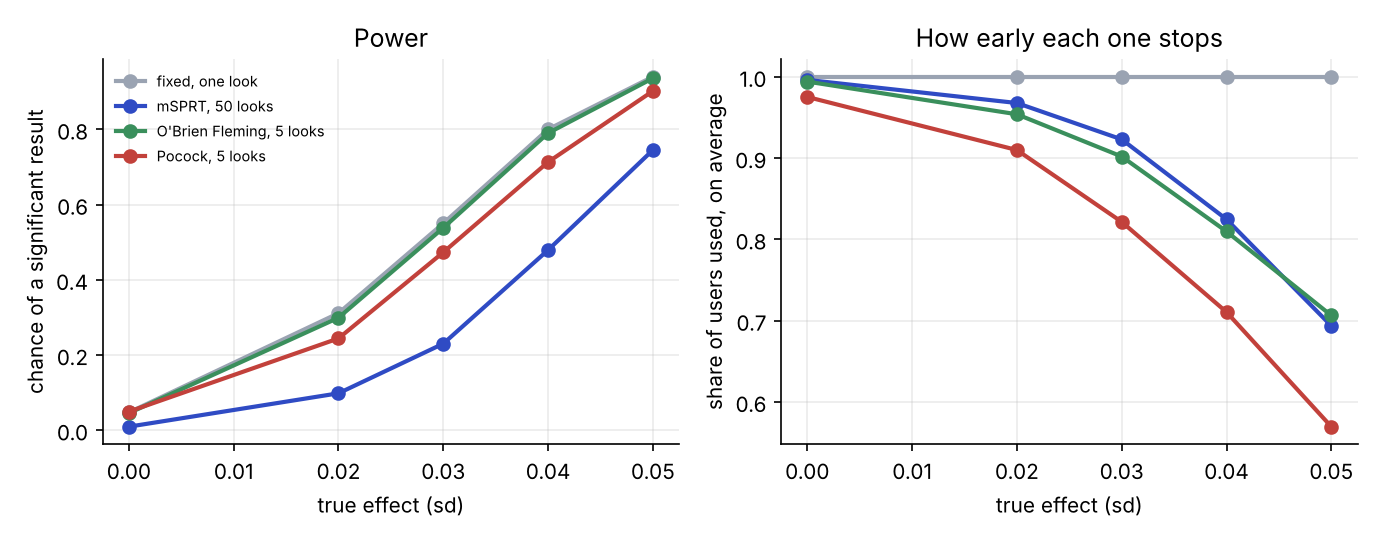
\includegraphics[width=0.88\linewidth]{../figures/gsd_tradeoff.png}
\caption{Power and stopping time for the four approaches.}
\label{fig:gsd}
\end{figure}

\section{CUPAC and why cross fitting matters}
The outcome is a nonlinear function of five pre period features plus noise, 1,500 users per group, 300 experiments with and 300 without an effect. Linear CUPED on the five features removes only 10\% of the variance, because the signal is nonlinear. Cross fitted CUPAC with gradient boosting removes 51\%, which nearly doubles power (48\% vs 26\%) with no detectable bias ($-0.5\% \pm 3.2\%$ of the effect) and a false positive rate of 4.7\%. Fitting the same model on all rows and predicting those same rows looks better on paper (75\% of the variance removed) but shrinks the estimated effect by 26\% ($\pm 2.2$), because part of each user's own outcome, treatment effect included, leaks into the covariate. Five nearest neighbors, where each user is one of their own neighbors, shrinks it by 22\%. The interval then misses the truth more often (91\% coverage). With 300 experiments per arm the Monte Carlo error on coverage is about 1.5 points, so the 92\% coverage of the cross fitted version is within noise of 95\%, but a larger run would be worth doing.

\begin{table}[!tb]
\centering\scriptsize
\begin{tabular}{lrrrrr}
\toprule
Method & Variance cut (\%) & Type I (\%) & Coverage (\%) & Bias (\% of effect) & Power (\%) \\
\midrule
No adjustment & 0 & 2.7 $\pm$ 0.9 & 94.7 $\pm$ 1.3 & -2 & 26 \\
CUPED, 5 linear covariates & 10 & 3.7 $\pm$ 1.1 & 92.0 $\pm$ 1.6 & -1 & 30 \\
CUPAC, cross fit & 51 & 4.7 $\pm$ 1.2 & 92.3 $\pm$ 1.5 & -1 & 48 \\
CUPAC, no cross fit (boosting) & 75 & 2.7 $\pm$ 0.9 & 90.7 $\pm$ 1.7 & -26 & 51 \\
CUPAC, no cross fit (5 neighbors) & 65 & 3.0 $\pm$ 1.0 & 91.3 $\pm$ 1.6 & -22 & 45 \\
\bottomrule
\end{tabular}

\caption{Variance reduction and validity of covariate adjustment. Type I and coverage in percent $\pm$ one Monte Carlo standard error.}
\label{tab:cupac}
\end{table}

\section{Case study: Cookie Cats}
Cookie Cats is a mobile puzzle game. In a public experiment, 90,189 new players were randomized to have the first progress gate at level 30 (control) or level 40. Outcomes are whether the player returned 1 and 7 days after installing, and the number of rounds played in the first two weeks (capped at the 99th percentile, 493 rounds, because one player logged almost 50,000).

\begin{table}[H]
\centering\small
\begin{tabular}{lrrrrr}
\toprule
Metric & Gate 30 & Gate 40 & Relative lift & 95\% CI & BH adjusted $p$ \\
\midrule
1 day retention & 44.8\% & 44.2\% & $-1.3\%$ & $-2.8\%$ to $+0.1\%$ & 0.112 \\
7 day retention & 19.0\% & 18.2\% & $-4.3\%$ & $-6.9\%$ to $-1.7\%$ & 0.005 \\
Rounds played (capped) & 49.1 & 48.9 & $-0.6\%$ & $-2.8\%$ to $+1.7\%$ & 0.615 \\
\bottomrule
\end{tabular}
\caption{Cookie Cats results on all players.}
\end{table}

\paragraph{The split check.} The groups have 44,700 and 45,489 players, a sample ratio mismatch with $p = 0.0086$ under the intended 50/50 split. A healthy test lands there about one time in 116, so a fair test can still land here. Teams that alert only below 0.001 would not have flagged it.

\paragraph{A placebo from the game design.} The gate is at level 30 or 40. A player with fewer than 29 rounds cannot have completed 29 levels (assuming at least one round per level), so they never reached either gate and played the same game in both versions. Their count per group and their retention cannot depend on the treatment. Among those players the split is 27,742 vs 28,565 ($p = 0.0005$); among players with 29 or more rounds it is 16,958 vs 16,924 ($p = 0.85$). The share of low activity players differs between groups (62.1\% vs 62.8\%, $p = 0.023$). Zero round players, the first suspect for an install logging problem, account for only 15\% of the excess. The buckets are not perfectly clean, since players with 29 to 39 rounds are split 3,392 vs 3,097 ($p = 0.00025$). I read that as the gate moving players around, because gate\_30 players stall near level 30, but a second problem cannot be ruled out. The pattern suggests extra or missing low engagement records in one group (install attribution, logging, exclusions) more than a skewed randomizer, and the data cannot show which. The 29 round cut came from the game design; other cuts, which I also examined, give the same picture.

\begin{figure}[!tb]
\centering
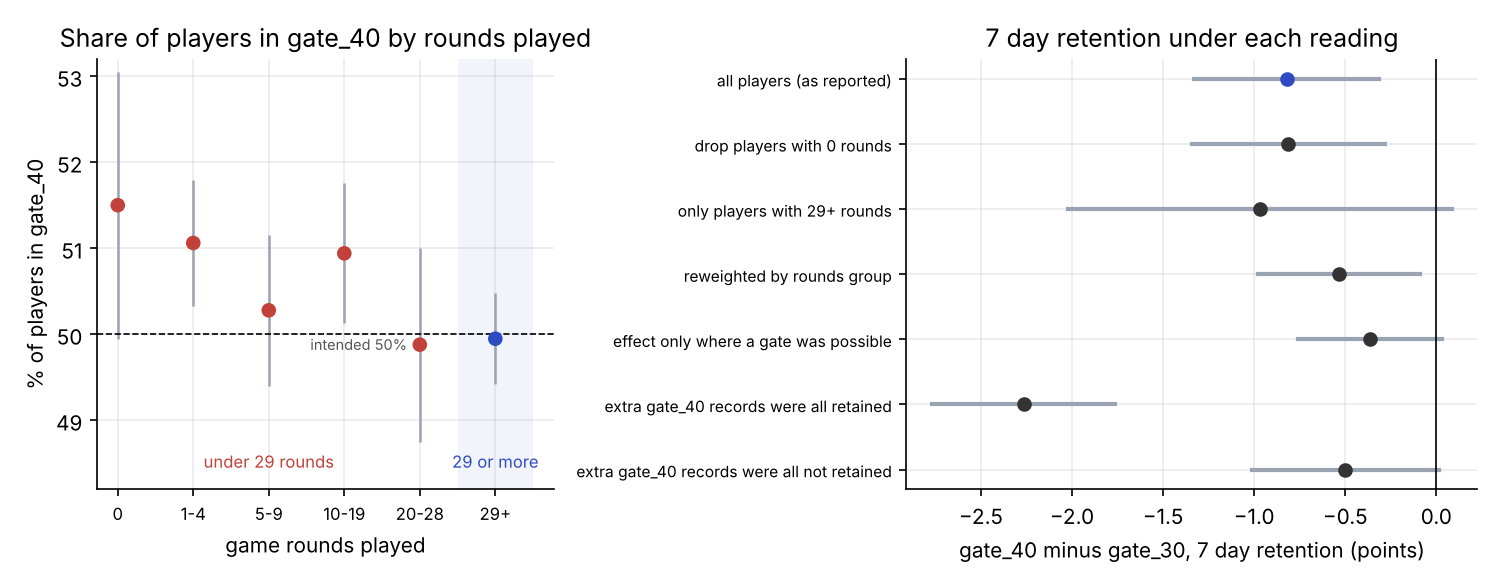
\includegraphics[width=\linewidth]{../figures/cookie_cats_srm.png}
\caption{Left: share of players in gate\_40 by rounds played, with 95\% intervals. Only the 29+ total is shown above the cut, because how players spread across 29 to 39 and 40+ rounds is itself moved by the gate. Right: the 7 day retention effect under the readings in Table~\ref{tab:srm}.}
\end{figure}

\paragraph{Sensitivity.} Table~\ref{tab:srm} shows the 7 day retention effect under different readings. Among players who never reached a gate, retention was 4.12\% vs 3.84\% ($-0.27$ points, $p = 0.098$), in the direction expected if gate\_40 contains extra low engagement records. An exact decomposition attributes $-0.29$ of the $-0.82$ point gap to the different mix of players, $-0.17$ to the difference within the low activity group and $-0.36$ to the players who could reach a gate.

\begin{table}[!tb]
\centering\small
\begin{tabular}{lrrr}
\toprule
Analysis & Change (points) & 95\% CI & $p$ \\
\midrule
all players (as reported) & $-0.82$ & $-1.33$ to $-0.31$ & 0.0016 \\
drop players with 0 rounds & $-0.81$ & $-1.34$ to $-0.28$ & 0.0026 \\
only players with 29+ rounds & $-0.97$ & $-2.02$ to $+0.08$ & 0.0711 \\
reweighted by rounds group & $-0.53$ & $-0.98$ to $-0.09$ & 0.0183 \\
effect only where a gate was possible & $-0.36$ & $-0.76$ to $+0.03$ & 0.0711 \\
extra gate\_40 records were all retained & $-2.26$ & $-2.77$ to $-1.76$ & $<$0.0001 \\
extra gate\_40 records were all not retained & $-0.50$ & $-1.01$ to $+0.01$ & 0.0561 \\
\bottomrule
\end{tabular}

\caption{7 day retention, gate\_40 minus gate\_30, under readings of the sample ratio mismatch. The last two rows are trimming bounds in the spirit of Lee (2009) that remove the 789 extra gate\_40 players with the most and least favorable outcomes.}
\label{tab:srm}
\end{table}

Every reading keeps the direction. In the subgroup with a clean split, the effect is a drop of about 1 point among players who could reach a gate, with $p = 0.07$. The reasonable conclusion is that moving the gate later probably lowered 7 day retention, that the subgroup $p$ of 0.07 reflects less data more than a smaller effect, since that subgroup is 38\% of the players and its estimate is a little larger, and that the assignment and install logs for low activity players should be checked before acting.

\paragraph{The sequential replay uses a shuffled order.} The data has no timestamps. Replaying the test as if it were checked 50 times therefore puts players in a random order, which shows how an always valid test behaves when arrival order is luck and nothing else; it cannot show anything that depends on time. Over 1,000 shuffles the mSPRT called the 7 day result every time, stopping after 22\% to 100\% of the players (5th to 95th percentile, median 78\%).

\section{Limitations}
The mSPRT guarantee uses a plug in variance and is asymptotic. The skewness note relies on a sample skewness, which is itself noisy for heavy tails. With very uneven cluster sizes and few clusters the $t$ version of \texttt{cluster\_test} still runs liberal, and only the randomization test came close to the right size. The sequential tests treat rows as independent. No method fixes missing data that depends on the outcome; the missing value check catches differential missingness but rarely catches outcome driven loss under the same rule in both groups. The relative interval reported after CUPED divides by the control mean as if it were known. Screening treats effects by quantile bins rather than modeling them. Nothing here handles interference between users. The Cookie Cats placebo assumes a level takes at least one round. Finally, the methods have been checked against software and published tables, but not yet reviewed by a statistician who didn't build them; \texttt{docs/review\_guide.md} lists the claims I would most like checked.

\section*{References}
\small
\begin{itemize}\setlength{\itemsep}{1pt}
\item Armitage, P., McPherson, C. K. and Rowe, B. C. (1969). Repeated significance tests on accumulating data. \textit{JRSS A}.
\item Benjamini, Y. and Hochberg, Y. (1995). Controlling the false discovery rate. \textit{JRSS B}.
\item Brunner, E. and Munzel, U. (2000). The nonparametric Behrens Fisher problem. \textit{Biometrical Journal}.
\item Deng, A., Xu, Y., Kohavi, R. and Walker, T. (2013). Improving the sensitivity of online controlled experiments by utilizing pre experiment data. \textit{WSDM}.
\item Deng, A., Knoblich, U. and Lu, J. (2018). Applying the delta method in metric analytics. \textit{KDD}.
\item Dunnett, C. W. (1955). A multiple comparison procedure for comparing several treatments with a control. \textit{JASA}.
\item Fabijan, A. et al. (2019). Diagnosing sample ratio mismatch in online controlled experiments. \textit{KDD}.
\item Howard, S., Ramdas, A., McAuliffe, J. and Sekhon, J. (2021). Time uniform, nonparametric, nonasymptotic confidence sequences. \textit{Annals of Statistics}.
\item Jennison, C. and Turnbull, B. W. (2000). \textit{Group Sequential Methods with Applications to Clinical Trials}. Chapman and Hall.
\item Johari, R., Koomen, P., Pekelis, L. and Walsh, D. (2017). Peeking at A/B tests. \textit{KDD}.
\item Kohavi, R., Deng, A., Longbotham, R. and Xu, Y. (2014). Seven rules of thumb for web site experimenters. \textit{KDD}.
\item Kohavi, R., Tang, D. and Xu, Y. (2020). \textit{Trustworthy Online Controlled Experiments}. Cambridge University Press.
\item Lan, K. K. G. and DeMets, D. L. (1983). Discrete sequential boundaries for clinical trials. \textit{Biometrika}.
\item Lee, D. S. (2009). Training, wages, and sample selection: estimating sharp bounds on treatment effects. \textit{Review of Economic Studies}.
\item Lin, W. (2013). Agnostic notes on regression adjustments to experimental data. \textit{Annals of Applied Statistics}.
\item O'Brien, P. C. and Fleming, T. R. (1979). A multiple testing procedure for clinical trials. \textit{Biometrics}.
\item Pocock, S. J. (1977). Group sequential methods in the design and analysis of clinical trials. \textit{Biometrika}.
\end{itemize}
\end{document}
